\qrchapter{https://forgottenpillar.com/rsc/en-fp-chapter2}{The Fundamental Principles}


\qrchapter{https://forgottenpillar.com/rsc/es-fp-chapter2}{Los Principios Fundamentales}


The real issue according to chapter ten of the Special Testimonies is diverting from the foundation of our faith, which was established at the beginning of our work.


El verdadero asunto, de acuerdo con el capítulo diez de los Testimonios Especiales, es desviarse del fundamento de nuestra fe, el cual fue establecido al principio de nuestra obra.


\egw{\textbf{This foundation was built by the Masterworker}, and \underline{will} stand storm and tempest. Will they permit this man to \textbf{present doctrines that deny the past experience} of the people of God? The time has come to take decided action.}[SpTB02 54.2; 1904][https://egwwritings.org/read?panels=p417.276]


\egw{\textbf{Este fundamento fue construido por el Maestro Trabajador}, y \underline{resistirá} tormenta y tempestad. ¿Permitirán que este hombre \textbf{presente doctrinas que niegan la experiencia pasada} del pueblo de Dios? Ha llegado el momento de tomar una acción decidida.}[SpTB02 54.2; 1904][https://egwwritings.org/read?panels=p417.276]


Kellogg presented doctrines that deny the past experience. In another place, she wrote about Kellogg:


Kellogg presentó doctrinas que niegan la experiencia pasada. En otro lugar, ella escribió sobre Kellogg:


\egw{I am much worried about Dr. Kellogg. In many respects, his course is not pleasing to the Lord. It seems to be \textbf{so easy for him to drift away from \underline{foundation principles}}. He is in great danger \textbf{of not holding the beginning of his confidence} steadfast unto the end.}[Lt138-1902.5; 1902][https://egwwritings.org/read?panels=p9219.11]


\egw{Estoy muy preocupada por el Dr. Kellogg. En muchos aspectos, su curso no agrada al Señor. Parece ser \textbf{tan fácil para él alejarse de los \underline{principios fundamentales}}. Está en gran peligro \textbf{de no mantener firme el principio de su confianza} hasta el final.}[Lt138-1902.5; 1902][https://egwwritings.org/read?panels=p9219.11]


The problem was the departing from the foundation principles—but not all people recognized that. Especially the key and prominent people in the work; they forgot the way the Lord led them and His teaching in the past.


El problema fue el alejamiento de los principios fundamentales, pero no todos lo reconocieron. Especialmente las personas clave y prominentes en la obra; olvidaron la forma en que el Señor los guió y su enseñanza en el pasado.


\egw{I have been hoping that there would be a thorough reformation, and that \textbf{the principles} for which we fought \textbf{in the early days}, and which were brought out in the power of the Holy Spirit, \textbf{would be maintained}.}[SpTB02 56.3; 1904][https://egwwritings.org/read?panels=p417.287]


\egw{He estado esperando que hubiera una reforma profunda, y que \textbf{los principios} por los que luchamos \textbf{en los primeros días}, y que fueron sacados a la luz con el poder del Espíritu Santo, \textbf{se mantuvieran}.}[SpTB02 56.3; 1904][https://egwwritings.org/read?panels=p417.287]


What were the principles that we fought for in the early days? What was this foundation of our faith?


¿Cuáles fueron los principios por los que luchamos en los primeros días? ¿Cuál era el fundamento de nuestra fe?


\egw{As a people, we are to \textbf{stand firm on the platform of eternal truth} that has withstood test and trial. We are to \textbf{hold to the sure pillars of our faith}. \textbf{The \underline{principles of truth}} that God has revealed to us \textbf{are our only true foundation}. They have made us what we are...}[SpTB02 51.2; 1904][https://egwwritings.org/read?panels=p417.261]


\egw{Como pueblo, debemos \textbf{mantenernos firmes en la plataforma de la verdad eterna} que ha resistido la prueba y el juicio. Debemos \textbf{aferrarnos a los pilares seguros de nuestra fe}. \textbf{Los \underline{principios de la verdad}} que Dios nos ha revelado \textbf{son nuestro único y verdadero fundamento}. Ellos nos han hecho lo que somos...}[SpTB02 51.2; 1904][https://egwwritings.org/read?panels=p417.261]


The \egwinline{principles of truth} that God has revealed \egwinline{is our only true foundation}. She is calling these principles the platform of eternal truth. She refers to these principles as the \egwinline{sure pillars of our faith}[SpTB02 51.2; 1904][https://egwwritings.org/read?panels=p417.261].


Los \egwinline{principios de la verdad} que Dios ha revelado \egwinline{son nuestro único y verdadero fundamento}. Ella llama a estos principios la plataforma de la verdad eterna. Se refiere a estos principios como los \egwinline{pilares seguros de nuestra fe}[SpTB02 51.2; 1904][https://egwwritings.org/read?panels=p417.261].


She recalls the past experience of our pioneers, like James White, Joseph Bates, Elder Edson, father Pierce, how God worked on them until \egwinline{point by point}, \egwinline{all \textbf{the principal points of our faith} were made clear}. She recalled how \egwinline{this foundation was built by the Masterworker,} and assures that it \egwinline{will stand storm and tempest}. In conclusion, she strongly affirms the will of God for us regarding these principles. God \egwinline{calls upon us to \textbf{hold firmly}, with the grip of faith, \textbf{to the fundamental principles that are based upon unquestionable authority}}.


Ella recuerda la experiencia pasada de nuestros pioneros, como James White, Joseph Bates, el anciano Edson, el padre Pierce, cómo Dios trabajó en ellos hasta que \egwinline{punto por punto}, \egwinline{todos \textbf{los puntos principales de nuestra fe} fueron aclarados}. Recordó cómo \egwinline{este fundamento fue construido por el Maestro obrero,} y asegura que \egwinline{resistirá tormenta y tempestad}. En conclusión, afirma con firmeza la voluntad de Dios para nosotros en relación con estos principios. Dios \egwinline{nos llama a \textbf{aferrarnos firmemente}, con la garra de la fe, \textbf{a los principios fundamentales que se basan en una autoridad incuestionable}}.


We see several different expressions that Sister White used for the foundation of our faith: “\textit{the platform of eternal truth},” “\textit{pillars of our faith},” “\textit{principles of truth},” “\textit{principal points},” “\textit{waymarks},” “\textit{foundation principles},” and “\textit{fundamental principles}”. These expressions denote the same thing—the foundation of our faith. When we hear these expressions today, somehow they don’t convey any concrete information. But for Seventh-day Adventists in her time, this was very clear and a definite point. All of these terms are referring to the public synopsis of Seventh-day Adventist’s faith called the \emcap{Fundamental Principles}, further explained below.


Vemos varias expresiones diferentes que la hermana White utilizó para el fundamento de nuestra fe: “\textit{la plataforma de la verdad eterna}”, “\textit{los pilares de nuestra fe}”, “\textit{los principios de la verdad}”, “\textit{los puntos principales}”, “\textit{hitos}”, “\textit{los principios fundacionales}” y “\textit{los principios fundamentales}”. Estas expresiones denotan lo mismo—el fundamento de nuestra fe. Cuando oímos estas expresiones hoy, de alguna manera no transmiten ninguna información concreta. Pero para los Adventistas del Séptimo Día en su tiempo, esto era muy claro y un punto definido. Todos estos términos se refieren a la sinopsis pública de la fe de los adventistas del séptimo día llamada \emcap{Principios Fundamentales}, que se explica más adelante.


God \egwinline{calls upon us to \textbf{hold firmly}, with the grip of faith, to \textbf{the \underline{fundamental principles}} that  are \textbf{based upon unquestionable authority}.} This is a reference to principal features of Seventh-day Adventist faith which God revealed to Adventist pioneers \egwinline{after the passing of the time in 1844,} when a group of keen, noble, and true men \egwinline{searched for the truth as for hidden treasure.} This was \textit{the foundation of our faith}. Our pioneers officially established the Seventh-day Adventist Church in 1863, and they taught these truths which they called “\textit{fundamental principles}.” But often, Seventh-day Adventists were misrepresented publicly. For this reason, in 1872, our pioneers published a document called “\textit{A Declaration of the Fundamental Principles, Taught and Practiced by the Seventh-day Adventists}” in order to publicly, but briefly, declare what \emcap{fundamental principles} Seventh-day Adventists taught and practiced. These \emcap{Fundamental Principles} were regularly printed as a standalone pamphlet, were present in our papers, and were annually printed in Adventist Yearbooks throughout Ellen White's lifetime.\footnote{See \hyperref[appendix:timeline]{Fundamental Principles - Timeline} for more details.} Therefore, when Ellen White referenced the “\textit{fundamental principles},” this was not a vague or opaque statement, since the Seventh-day Adventist church had officially and publicly declared what these \emcap{fundamental principles} were. In the preface of this document, we read the purpose behind this document.


Dios \egwinline{nos llama a \textbf{aferrarnos firmemente}, con la garra de la fe, a \textbf{los \underline{principios fundamentales}} que \textbf{se basan en una autoridad incuestionable}.} Esta es una referencia a las características principales de la fe Adventista del Séptimo Día que Dios reveló a los pioneros adventistas \egwinline{después del paso del tiempo en 1844,} cuando un grupo de hombres agudos, nobles y verdaderos \egwinline{buscaron la verdad como un tesoro escondido.} Este fue \textit{el fundamento de nuestra fe}. Nuestros pioneros establecieron oficialmente la Iglesia Adventista del Séptimo Día en 1863, y enseñaron estas verdades que llamaron “\textit{principios fundamentales}.” Pero a menudo, los Adventistas del Séptimo Día eran mal representados públicamente. Por esta razón, en 1872, nuestros pioneros publicaron un documento llamado “\textit{Declaración de los Principios Fundamentales, Enseñados y Practicados por los Adventistas del Séptimo Día}” para declarar pública, pero brevemente, qué \emcap{principios fundamentales} enseñaban y practicaban los Adventistas del Séptimo Día. Estos \emcap{Principios Fundamentales} se imprimían regularmente como un folleto independiente, estaban presentes en nuestros periódicos y se imprimían anualmente en los Anuarios Adventistas durante toda la vida de Ellen White.\footnote{Ver \hyperref[appendix:timeline]{Principios Fundamentales - Cronología} para más detalles.} Por lo tanto, cuando Ellen White hacía referencia a los “\textit{principios fundamentales}”, esta no era una declaración vaga u opaca, ya que la iglesia Adventista del Séptimo Día había declarado oficial y públicamente cuáles eran estos \emcap{principios fundamentales}. En el prefacio de este documento, leemos el propósito detrás de este documento.


\begin{figure}
    \centering
    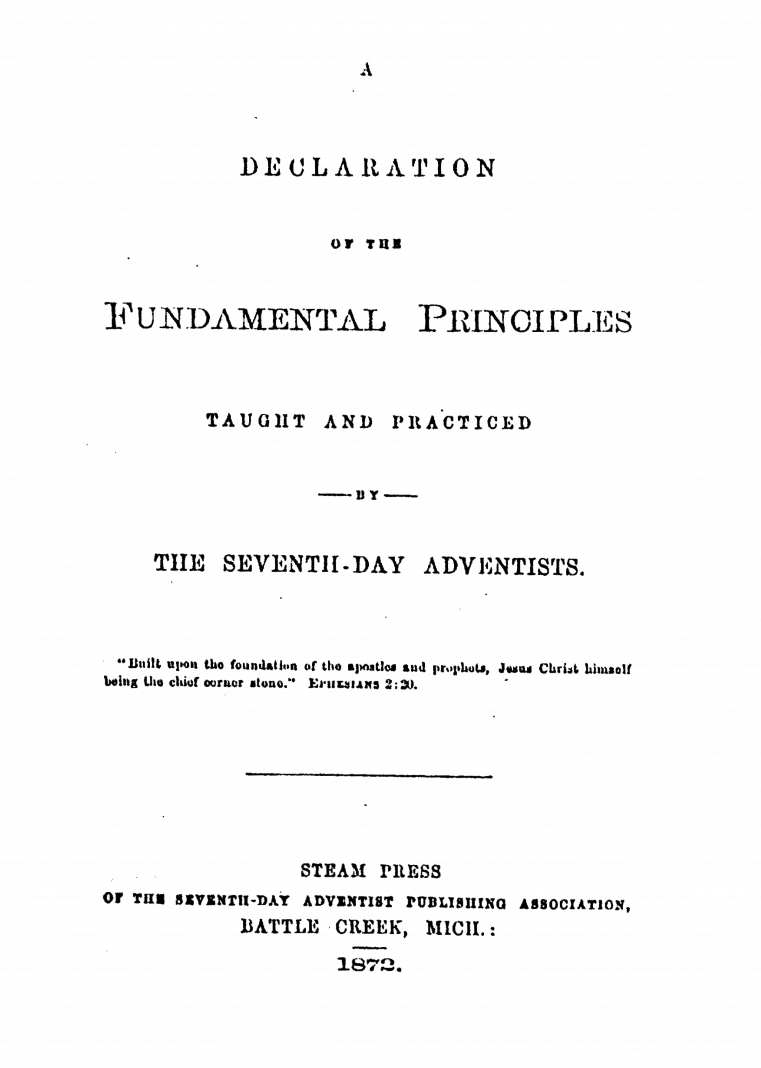
\includegraphics[width=1\linewidth]{images/declaration-of-the-fundamental-principles.PNG}
    \caption*{Scan of the Declaration of the Fundamental Principles, 1872.}
    \label{fig:declaration-of-the-fundamental-principles}
\end{figure}


\begin{figure}
    \centering
    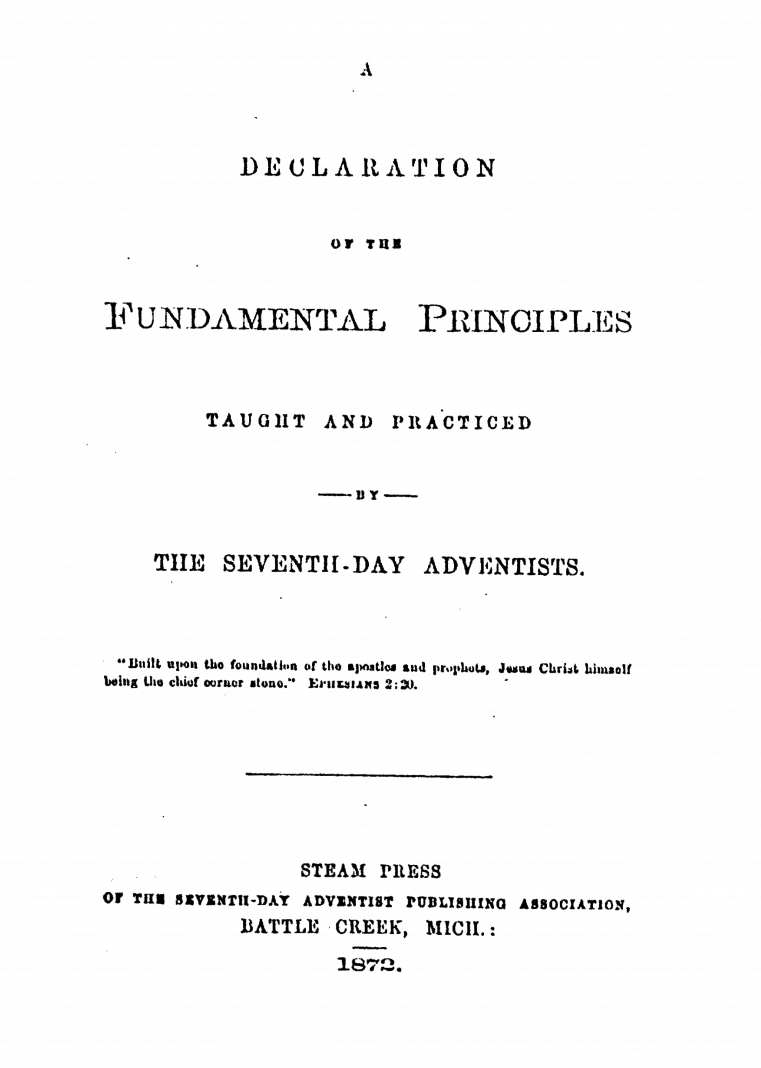
\includegraphics[width=1\linewidth]{images/declaration-of-the-fundamental-principles.PNG}
    \caption*{Escaneo de la Declaración de los Principios Fundamentales, 1872.}
    \label{fig:declaration-of-the-fundamental-principles}
\end{figure}


\others{In presenting to the \textbf{public} this \textbf{synopsis of our faith}, we wish to have it distinctly understood that \textbf{we have no articles of faith, creed, or discipline, }\textbf{\underline{aside from the Bible}}. We \textbf{do not} put forth this as \textbf{having any authority with our people}, \textbf{nor is it designed to secure uniformity among them}, \textbf{as a system of faith}, \textbf{but is a brief statement of \underline{what is, and has been, with great unanimity, held by them}}. We often find it necessary to meet inquiries on this subject, and sometimes to correct false statements circulated against us, and to remove erroneous impressions which have obtained with those who have not had an opportunity to become acquainted with our faith and practice. Our only object is to meet this necessity.}


\others{Al presentar al \textbf{público} esta \textbf{sinopsis de nuestra fe}, deseamos que se entienda claramente que \textbf{no tenemos artículos de fe, credo o disciplina, }\textbf{\underline{aparte de la Biblia}}. \textbf{No} presentamos esto como si \textbf{tuviera alguna autoridad entre nuestra gente}, \textbf{ni está diseñado para asegurar la uniformidad entre ellos}, \textbf{como un sistema de fe}, \textbf{sino que es una breve declaración de \underline{lo que es, y ha sido, con gran unanimidad, sostenido por ellos}}. A menudo nos encontramos con la necesidad de responder a las preguntas sobre este tema, y a veces corregir las falsas declaraciones que circulan contra nosotros, y eliminar las impresiones erróneas que han obtenido aquellos que no han tenido la oportunidad de conocer nuestra fe y práctica. Nuestro único objetivo es satisfacer esta necesidad.}


\othersnogap{\textbf{As Seventh-day Adventists we desire simply that our position shall be understood}; and we are the more solicitous for this because there are many who call themselves Adventists who hold views with which we can have no sympathy, some of which, we think, are subversive of the plainest and most important principles set forth in the word of God...}[The Fundamental Principles 1872, p. 3.1][https://egwwritings.org/read?panels=p928.8]


\othersnogap{\textbf{Como Adventistas del Séptimo Día deseamos simplemente que se comprenda nuestra posición}; y estamos más interesados en ello porque hay muchos que se llaman adventistas que sostienen puntos de vista con los que no podemos simpatizar, algunos de los cuales, pensamos, son subversivos de los principios más claros e importantes establecidos en la palabra de Dios...}[The Fundamental Principles 1872, p. 3.1][https://egwwritings.org/read?panels=p928.8]


This synopsis of faith consisted of 25 points, which represented \others{what is, and has been, with great unanimity, held by} Seventh-day Adventists. These 25 points constituted \egwinline{\textbf{the foundation} that was \textbf{laid at the beginning} of our work \textbf{by prayerful study} of the word and by revelation}. In 1904, Sister White told us that \egwinline{upon \textbf{this foundation} we have been building for \textbf{the past fifty years}.} These are the \egwinline{\textbf{the fundamental principles that are based upon unquestionable authority}}, that God \egwinline{calls upon us to \textbf{hold firmly}, with the grip of faith}. In other words, she repeated, \egwinline{we are to \textbf{hold to the sure pillars of our faith}}.


Esta sinopsis de fe consistía en 25 puntos, que representaban \others{lo que es, y ha sido, con gran unanimidad, sostenido por} los Adventistas del Séptimo Día. Estos 25 puntos constituían \egwinline{\textbf{el fundamento} que se puso \textbf{al principio} de nuestra obra \textbf{mediante el estudio en oración} de la palabra y por revelación}. En 1904, la hermana White nos dijo que \egwinline{sobre \textbf{este fundamento} hemos estado construyendo durante \textbf{los últimos cincuenta años}}. Estos son los \egwinline{\textbf{principios fundamentales que se basan en una autoridad incuestionable}}, que Dios \egwinline{nos llama a \textbf{aferrarnos firmemente}, con la garra de la fe}. En otras palabras, repitió, \egwinline{debemos \textbf{aferrarnos a los pilares seguros de nuestra fe}}.


In 1904, Sister White wrote about\egwinline{the \textbf{efforts of the enemy to undermine the foundation of our faith}}. She wrote about the movement that would\egwinline{consist in \textbf{giving up} the doctrines which stand as \textbf{the pillars of our faith}}. This reformation, if accepted, would discard\egwinline{\textbf{the principles of truth} that God in His wisdom has given to the remnant church} and\egwinline{\textbf{the fundamental principles} that have sustained the work for the last fifty years \textbf{would be accounted as error}}. This movement started about the time when Dr. John H. Kellogg published the book, “Living Temple”.


En 1904, la hermana White escribió sobre \egwinline{los \textbf{esfuerzos del enemigo para socavar el fundamento de nuestra fe}}. Escribió sobre el movimiento que \egwinline{consistiría en \textbf{abandonar} las doctrinas que se mantienen como \textbf{pilares de nuestra fe}}. Esta reforma, de ser aceptada, descartaría \egwinline{\textbf{los principios de la verdad} que Dios, en su sabiduría, ha dado a la iglesia remanente} y \egwinline{\textbf{los principios fundamentales} que han sostenido la obra durante los últimos cincuenta años \textbf{serían considerados como erróneos}}. Este movimiento comenzó más o menos cuando el Dr. John H. Kellogg publicó el libro, “Living Temple”.


\egw{About the time that ‘Living Temple’ was published, there passed before me in the night season, \textbf{representations indicating that some danger was approaching}, and that I must prepare for it by \textbf{writing out the things} God has revealed to me \textbf{regarding \underline{the foundation principles of our faith}}.}[SpTB02 52.3; 1904][https://egwwritings.org/read?panels=p417.267]


\egw{Alrededor del tiempo en que se publicó ‘Living Temple’, pasaron ante mí, en la estación nocturna, \textbf{representaciones que indicaban que se acercaba algún peligro}, y que debía prepararme para él \textbf{escribiendo} las cosas que Dios me había revelado \textbf{con respecto a \underline{los principios fundamentales de nuestra fe}}.}[SpTB02 52.3; 1904][https://egwwritings.org/read?panels=p417.267]


By publishing “Living Temple”, \textbf{foundation principles of our faith} \textbf{would be undermined}\egwinline{through the dissemination of \textbf{seductive theories}} contained therein.


Al publicar “Living Temple”, \textbf{los principios fundamentales de nuestra fe} \textbf{serían socavados} \egwinline{a través de la difusión de \textbf{teorías seductoras}} contenidas en el mismo.


\egw{I have been instructed by the heavenly messenger that some of the reasoning in the book, ‘Living Temple,’ is unsound and that \textbf{this reasoning would lead astray} the minds of those who are not thoroughly established on \textbf{the foundation principles} of present truth. It introduces that which is naught but speculation in \textbf{regard to \underline{the personality of God and where His presence is}}.}[SpTB02 51.3; 1904][https://egwwritings.org/read?panels=p417.262]


\egw{He sido instruida por el mensajero celestial que algunos de los razonamientos en el libro, ‘Living Temple,’ no son sólidos y que \textbf{este razonamiento desviaría} las mentes de aquellos que no están completamente establecidos en \textbf{los principios fundacionales} de la verdad presente. Introduce lo que no es más que especulación en \textbf{relación a \underline{la personalidad de Dios y dónde está su presencia}}.}[SpTB02 51.3; 1904][https://egwwritings.org/read?panels=p417.262]


Sister White is very particular in pointing out that the reasoning contained in the book Living Temple,\egwinline{\textbf{would lead astray}} from the\egwinline{\textbf{the foundation principles} of present truth}. These reasonings are in\egwinline{\textbf{regard to the personality of God and where His presence is}}.


La hermana White es muy particular al señalar que el razonamiento contenido en el libro Living Temple,\egwinline{\textbf{desviaría}} de\egwinline{\textbf{los principios fundacionales} de la verdad presente}. Estos razonamientos se refieren\egwinline{\textbf{a la personalidad de Dios y dónde está su presencia}}.


As mentioned before, the word ‘\textit{personality’}, in the context of the nineteenth century, is defined as “\textit{the quality or state of being a person}”\footnote{\href{https://www.merriam-webster.com/dictionary/personality}{Merriam-Webster Dictionary}, word ‘\textit{personality}’}. In other words, this term conveys the answer to the question, “\textit{what is it that defines someone to be a person?}”, “\textit{What is the quality or state of someone being a person?}” In the case of the \emcap{personality of God}, the question is, “\textit{Is God a person and what is it that defines Him as being a person? What is the quality or state of God being a person?}”


Como se mencionó anteriormente, la palabra ‘\textit{personalidad}’, en el contexto del siglo XIX, se define como “\textit{la cualidad o estado de ser una persona}”\footnote{\href{https://www.merriam-webster.com/dictionary/personality}{Merriam-Webster Dictionary}, palabra ‘\textit{personalidad}’}. En otras palabras, este término transmite la respuesta a la pregunta, “\textit{¿qué es lo que define a alguien como persona?}”, “\textit{¿Cuál es la cualidad o estado de alguien siendo una persona?}” En el caso de la \emcap{personalidad de Dios}, la pregunta es, “\textit{¿Es Dios una persona y qué es lo que lo define como tal? ¿Cuál es la cualidad o estado de Dios siendo una persona?}”


The reasoning of Dr. Kellogg regarding these questions expressed in the book Living Temple, is\egwinline{unsound}. The sentiments, in\egwinline{\textbf{regard to the personality of God and where His presence is}},\egwinline{advocated in the book, did not bear the indorsement of God, and that they were \textbf{a snare that the enemy had prepared for the last days}}. As we are living in the last days, we ought to ask ourselves these questions. Likewise, we are to question the biblical validity of the statements in the \emcap{Fundamental Principles} regarding the \emcap{personality of God} and where His presence is. How do the \emcap{Fundamental Principles} define God as being a person, and what do they say regarding God’s presence?


El razonamiento del Dr. Kellogg respecto a estas preguntas expresado en el libro Living Temple, es\egwinline{poco sólido}. Los sentimientos, en\egwinline{\textbf{lo que respecta a la personalidad de Dios y dónde está su presencia}},\egwinline{defendidos en el libro, no llevaban el aval de Dios, y eran \textbf{una trampa que el enemigo había preparado para los últimos días}}. Como estamos viviendo en los últimos días, debemos hacernos estas preguntas. Asimismo, debemos cuestionar la validez bíblica de las afirmaciones de los \emcap{Principios Fundamentales} respecto a la \emcap{personalidad de Dios} y dónde está su presencia. ¿Cómo definen los \emcap{Principios Fundamentales} a Dios como una persona, y qué dicen respecto a la presencia de Dios?


The first point listed below deals with the \emcap{personality of God} and His presence. The second point gives the context to the first. Please consider a few questions while reading them: Who is referred to as one God? How is God defined as a person or in other words, what is the quality or state of Him being a person? How do these points talk about the presence of God?


El primer punto que se menciona a continuación se refiere a la \emcap{personalidad de Dios} y a su presencia. El segundo punto da el contexto al primero. Por favor, considera algunas preguntas mientras los lees: ¿A quién se refiere como un Dios único? ¿Cómo se define a Dios como persona o, en otras palabras, cuál es la cualidad o estado de que sea una persona? ¿Cómo hablan estos puntos de la presencia de Dios?


\others{“I – That there is \textbf{one God}, \textbf{\underline{a personal, spiritual being}}, \textbf{the creator of all things}, omnipotent, omniscient, and eternal, infinite in wisdom, holiness, justice, goodness, truth, and mercy; unchangeable, and \textbf{\underline{everywhere present by his representative, the Holy Spirit}}. Ps. 139:7.”}


\others{“I – Que hay \textbf{un solo Dios}, \textbf{\underline{un ser personal y espiritual}}, \textbf{el creador de todas las cosas}, omnipotente, omnisciente y eterno, infinito en sabiduría, santidad, justicia, bondad, verdad y misericordia; inmutable, y \textbf{\underline{presente en todas partes por medio de su representante, el Espíritu Santo}}. Sal. 139:7.”}


\othersnogap{II – That there is \textbf{one Lord Jesus Christ, }\textbf{\underline{the Son of the Eternal Father}}, the one \textbf{\underline{by}}\textbf{ whom God created all things}, and by whom they do consist; …”}[The Fundamental Principles 1889, point no. 1.,2.,.] \footnote{See \hyperref[chap:appendix]{Appendix} for the full list of the Fundamental Principles} \footnote{From 1872 until 1914, the Fundamental Principles remained constant and unchanged, with the exception in 1889, when James Smith added three new points. But during all those years, the points concerning “\textit{the personality of God}” and “\textit{where His presence is}” remained the same. }


\othersnogap{II – Que hay \textbf{un solo Señor Jesucristo, }\textbf{\underline{el Hijo del Padre Eterno}}, aquel \textbf{\underline{por}}\textbf{ quien Dios creó todas las cosas}, y por quien éstas consisten; …“}[Los Principios Fundamentales 1889, punto no. 1.,2.,.] \footnote{Ver \hyperref[chap:appendix]{Apéndice} para la lista completa de los Principios Fundamentales} \footnote{Desde 1872 hasta 1914, los Principios Fundamentales permanecieron constantes e inalterados, con la excepción de 1889, cuando James Smith añadió tres nuevos puntos. Pero durante todos esos años, los puntos concernientes a “\textit{la personalidad de Dios}” y “\textit{dónde está su presencia}” permanecieron iguales. }


In the time of Ellen White, Seventh-day Adventists believed in one God—a personal, spiritual being, the Creator of all things—and they believed that this God created everything by His Son Jesus Christ. They addressed the Father as one God, and they addressed Christ as the Son of God. The quality or state of God being a person is expressed in the term “\textit{personal, spiritual being}”. Regarding His presence, the \emcap{Fundamental Principles} state that He is everywhere present by His representative, the Holy Spirit. The meaning of these principles requires very special attention. Keeping within the historical context, this will be the subject of our following studies.


En el tiempo de Ellen White, los Adventistas del Séptimo Día creían en un solo Dios—un ser personal y espiritual, el Creador de todas las cosas—y creían que este Dios creó todo por medio de su Hijo Jesucristo. Se dirigían al Padre como un solo Dios, y se dirigían a Cristo como el Hijo de Dios. La cualidad o estado de que Dios es una persona se expresa en el término “\textit{un ser personal y espiritual}”. En cuanto a su presencia, los \emcap{Principios Fundamentales} afirman que Él está presente en todas partes por medio de su representante, el Espíritu Santo. El significado de estos principios requiere una atención muy especial. Manteniéndonos dentro del contexto histórico, éste será el tema de nuestros siguientes estudios.


\section*{The Test}


\section*{La Prueba}


Most obviously, these \emcap{fundamental principles} do not contain the doctrine of the Trinity! More precisely, the sentiments “\textit{three in one},” or “\textit{one in three}”, in reference to God, are nowhere to be found—which are present in today’s \textit{Fundamental Beliefs}. Only the Father is referred to as “\textit{one God’‘}. But before rushing to swift conclusions, and condemning the doctrine of the Trinity as\egwinline{\textbf{seductive theories,}} which\egwinline{\textbf{undermine the foundation of our faith}}, please bear in mind that Sister White presents a comprehensive list of characteristics that must be fulfilled in order for it to be deemed as such.


Lo más evidente es que estos \emcap{principios fundamentales} no contienen la doctrina trinitaria! Más precisamente, los sentimientos “\textit{tres en uno},” o “\textit{uno en tres}”, en referencia a Dios, no se encuentran en ninguna parte—que están presentes en las \textit{Creencias Fundamentales} de hoy. Sólo se habla del Padre como “\textit{un solo Dios’‘}. Pero antes de apresurarse a sacar conclusiones rápidas, y condenar la doctrina trinitaria como\egwinline{\textbf{teorías seductoras,}} que\egwinline{\textbf{socavan el fundamento de nuestra fe}}, por favor, tenga en cuenta que la hermana White presenta una lista exhaustiva de características que deben cumplirse para que sea considerada como tal.


If the Trinity doctrine is questionable, then the trinitarian sentiments would need to:
\begin{itemize}
    \item rob the people of God of their past experience
    \item destroy the \emcap{personality of God}
    \item tear down the pillars of our faith or lead astray from the foundation principles
    \item be presented as if Mrs. White supported them
\end{itemize}


Si la doctrina trinitaria es cuestionable, entonces los sentimientos trinitarios tendrían que:
\begin{itemize}
    \item despojar al pueblo de Dios de su experiencia pasada
    \item destruir la \emcap{personalidad de Dios}
    \item derribar los pilares de nuestra fe o desviarse de los principios fundamentales
    \item ser presentados como si la Sra. White los apoyara
\end{itemize}


It is not our intention to deal with any of Kellogg’s seductive theories, but rather to study the \emcap{personality of God} in its historical background. As we do this, we will face the evidence of Sister White reactively warning the church of these characteristics.


No es nuestra intención tratar ninguna de las seductoras teorías de Kellogg, sino estudiar la \emcap{personalidad de Dios} en su trasfondo histórico. Al hacerlo, nos enfrentaremos a la evidencia de que la hermana White advirtió reactivamente a la iglesia de estas características.


% The Fundamental Prinicples

\begin{titledpoem}
    \stanza{
        The Masterworker built a foundation strong, \\
        To guide God's people as they journey long. \\
        These truths revealed through prayer and earnest toil, \\
        Stand firm on heaven's unquestionable soil.
    }

    \stanza{
        God as one personal and spiritual being, \\
        Present through His Spirit, all-knowing, all-seeing. \\
        Christ as the Son of the Eternal Father, \\
        These pillars of faith we should hold, not bother.
    }

    \stanza{
        When men depart from these principles true, \\
        Undermining foundations through teachings new, \\
        The wisdom of ages they quickly discard, \\
        And God's revealed pathway becomes sadly marred.
    }

    \stanza{
        Hold firmly the truth with unwavering grip, \\
        Let not from these anchors your faith ever slip. \\
        For what God established through pioneers' hands, \\
        Through tempest and storm eternally stands.
    }
\end{titledpoem}


% \qrchapter{https://forgottenpillar.com/rsc/en-fp-chapter2}{The Fundamental Principles}

The real issue according to chapter ten of the Special Testimonies is diverting from the foundation of our faith, which was established at the beginning of our work.

\egw{\textbf{This foundation was built by the Masterworker}, and \underline{will} stand storm and tempest. Will they permit this man to \textbf{present doctrines that deny the past experience} of the people of God? The time has come to take decided action.}[SpTB02 54.2; 1904][https://egwwritings.org/read?panels=p417.276]

Kellogg presented doctrines that deny the past experience. In another place, she wrote about Kellogg:

\egw{I am much worried about Dr. Kellogg. In many respects, his course is not pleasing to the Lord. It seems to be \textbf{so easy for him to drift away from \underline{foundation principles}}. He is in great danger \textbf{of not holding the beginning of his confidence} steadfast unto the end.}[Lt138-1902.5; 1902][https://egwwritings.org/read?panels=p9219.11]

The problem was the departing from the foundation principles—but not all people recognized that. Especially the key and prominent people in the work; they forgot the way the Lord led them and His teaching in the past. 

\egw{I have been hoping that there would be a thorough reformation, and that \textbf{the principles} for which we fought \textbf{in the early days}, and which were brought out in the power of the Holy Spirit, \textbf{would be maintained}.}[SpTB02 56.3; 1904][https://egwwritings.org/read?panels=p417.287]

What were the principles that we fought for in the early days? What was this foundation of our faith?

\egw{As a people, we are to \textbf{stand firm on the platform of eternal truth} that has withstood test and trial. We are to \textbf{hold to the sure pillars of our faith}. \textbf{The \underline{principles of truth}} that God has revealed to us \textbf{are our only true foundation}. They have made us what we are...}[SpTB02 51.2; 1904][https://egwwritings.org/read?panels=p417.261]

The \egwinline{principles of truth} that God has revealed \egwinline{is our only true foundation}. She is calling these principles the platform of eternal truth. She refers to these principles as the \egwinline{sure pillars of our faith}[SpTB02 51.2; 1904][https://egwwritings.org/read?panels=p417.261]. 

She recalls the past experience of our pioneers, like James White, Joseph Bates, Elder Edson, father Pierce, how God worked on them until \egwinline{point by point}, \egwinline{all \textbf{the principal points of our faith} were made clear}. She recalled how \egwinline{this foundation was built by the Masterworker,} and assures that it \egwinline{will stand storm and tempest}. In conclusion, she strongly affirms the will of God for us regarding these principles. God \egwinline{calls upon us to \textbf{hold firmly}, with the grip of faith, \textbf{to the fundamental principles that are based upon unquestionable authority}}. 

We see several different expressions that Sister White used for the foundation of our faith: “\textit{the platform of eternal truth},” “\textit{pillars of our faith},” “\textit{principles of truth},” “\textit{principal points},” “\textit{waymarks},” “\textit{foundation principles},” and “\textit{fundamental principles}”. These expressions denote the same thing—the foundation of our faith. When we hear these expressions today, somehow they don’t convey any concrete information. But for Seventh-day Adventists in her time, this was very clear and a definite point. All of these terms are referring to the public synopsis of Seventh-day Adventist’s faith called the \emcap{Fundamental Principles}, further explained below.

God \egwinline{calls upon us to \textbf{hold firmly}, with the grip of faith, to \textbf{the \underline{fundamental principles}} that  are \textbf{based upon unquestionable authority}.} This is a reference to principal features of Seventh-day Adventist faith which God revealed to Adventist pioneers \egwinline{after the passing of the time in 1844,} when a group of keen, noble, and true men \egwinline{searched for the truth as for hidden treasure.} This was \textit{the foundation of our faith}. Our pioneers officially established the Seventh-day Adventist Church in 1863, and they taught these truths which they called “\textit{fundamental principles}.” But often, Seventh-day Adventists were misrepresented publicly. For this reason, in 1872, our pioneers published a document called “\textit{A Declaration of the Fundamental Principles, Taught and Practiced by the Seventh-day Adventists}” in order to publicly, but briefly, declare what \emcap{fundamental principles} Seventh-day Adventists taught and practiced. These \emcap{Fundamental Principles} were regularly printed as a standalone pamphlet, were present in our papers, and were annually printed in Adventist Yearbooks throughout Ellen White's lifetime.\footnote{See \hyperref[appendix:timeline]{Fundamental Principles - Timeline} for more details.} Therefore, when Ellen White referenced the “\textit{fundamental principles},” this was not a vague or opaque statement, since the Seventh-day Adventist church had officially and publicly declared what these \emcap{fundamental principles} were. In the preface of this document, we read the purpose behind this document.

\begin{figure}
    \centering
    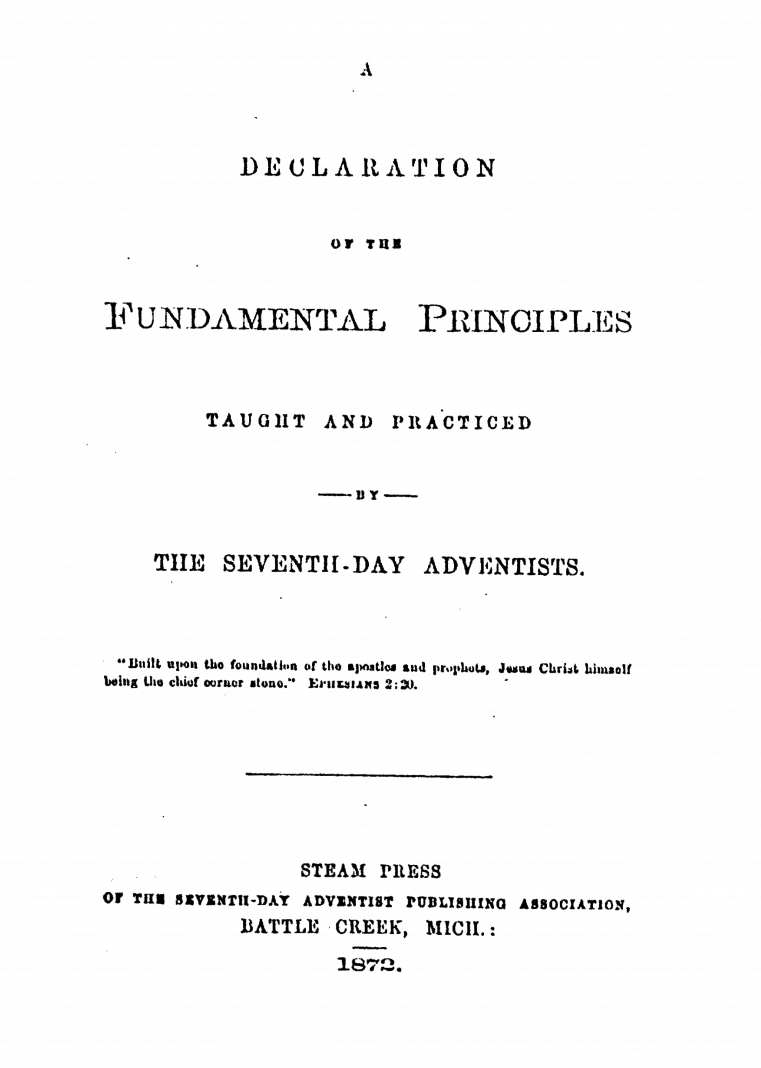
\includegraphics[width=1\linewidth]{images/declaration-of-the-fundamental-principles.PNG}
    \caption*{Scan of the Declaration of the Fundamental Principles, 1872.}
    \label{fig:declaration-of-the-fundamental-principles}
\end{figure}

\others{In presenting to the \textbf{public} this \textbf{synopsis of our faith}, we wish to have it distinctly understood that \textbf{we have no articles of faith, creed, or discipline, }\textbf{\underline{aside from the Bible}}. We \textbf{do not} put forth this as \textbf{having any authority with our people}, \textbf{nor is it designed to secure uniformity among them}, \textbf{as a system of faith}, \textbf{but is a brief statement of \underline{what is, and has been, with great unanimity, held by them}}. We often find it necessary to meet inquiries on this subject, and sometimes to correct false statements circulated against us, and to remove erroneous impressions which have obtained with those who have not had an opportunity to become acquainted with our faith and practice. Our only object is to meet this necessity.}

\othersnogap{\textbf{As Seventh-day Adventists we desire simply that our position shall be understood}; and we are the more solicitous for this because there are many who call themselves Adventists who hold views with which we can have no sympathy, some of which, we think, are subversive of the plainest and most important principles set forth in the word of God...}[The Fundamental Principles 1872, p. 3.1][https://egwwritings.org/read?panels=p928.8]

This synopsis of faith consisted of 25 points, which represented \others{what is, and has been, with great unanimity, held by} Seventh-day Adventists. These 25 points constituted \egwinline{\textbf{the foundation} that was \textbf{laid at the beginning} of our work \textbf{by prayerful study} of the word and by revelation}. In 1904, Sister White told us that \egwinline{upon \textbf{this foundation} we have been building for \textbf{the past fifty years}.} These are the \egwinline{\textbf{the fundamental principles that are based upon unquestionable authority}}, that God \egwinline{calls upon us to \textbf{hold firmly}, with the grip of faith}. In other words, she repeated, \egwinline{we are to \textbf{hold to the sure pillars of our faith}}.

In 1904, Sister White wrote about\egwinline{the \textbf{efforts of the enemy to undermine the foundation of our faith}}. She wrote about the movement that would\egwinline{consist in \textbf{giving up} the doctrines which stand as \textbf{the pillars of our faith}}. This reformation, if accepted, would discard\egwinline{\textbf{the principles of truth} that God in His wisdom has given to the remnant church} and\egwinline{\textbf{the fundamental principles} that have sustained the work for the last fifty years \textbf{would be accounted as error}}. This movement started about the time when Dr. John H. Kellogg published the book, “Living Temple”.

\egw{About the time that ‘Living Temple’ was published, there passed before me in the night season, \textbf{representations indicating that some danger was approaching}, and that I must prepare for it by \textbf{writing out the things} God has revealed to me \textbf{regarding \underline{the foundation principles of our faith}}.}[SpTB02 52.3; 1904][https://egwwritings.org/read?panels=p417.267]

By publishing “Living Temple”, \textbf{foundation principles of our faith} \textbf{would be undermined}\egwinline{through the dissemination of \textbf{seductive theories}} contained therein. 

\egw{I have been instructed by the heavenly messenger that some of the reasoning in the book, ‘Living Temple,’ is unsound and that \textbf{this reasoning would lead astray} the minds of those who are not thoroughly established on \textbf{the foundation principles} of present truth. It introduces that which is naught but speculation in \textbf{regard to \underline{the personality of God and where His presence is}}.}[SpTB02 51.3; 1904][https://egwwritings.org/read?panels=p417.262]

Sister White is very particular in pointing out that the reasoning contained in the book Living Temple,\egwinline{\textbf{would lead astray}} from the\egwinline{\textbf{the foundation principles} of present truth}. These reasonings are in\egwinline{\textbf{regard to the personality of God and where His presence is}}.

As mentioned before, the word ‘\textit{personality’}, in the context of the nineteenth century, is defined as “\textit{the quality or state of being a person}”\footnote{\href{https://www.merriam-webster.com/dictionary/personality}{Merriam-Webster Dictionary}, word ‘\textit{personality}’}. In other words, this term conveys the answer to the question, “\textit{what is it that defines someone to be a person?}”, “\textit{What is the quality or state of someone being a person?}” In the case of the \emcap{personality of God}, the question is, “\textit{Is God a person and what is it that defines Him as being a person? What is the quality or state of God being a person?}”

The reasoning of Dr. Kellogg regarding these questions expressed in the book Living Temple, is\egwinline{unsound}. The sentiments, in\egwinline{\textbf{regard to the personality of God and where His presence is}},\egwinline{advocated in the book, did not bear the indorsement of God, and that they were \textbf{a snare that the enemy had prepared for the last days}}. As we are living in the last days, we ought to ask ourselves these questions. Likewise, we are to question the biblical validity of the statements in the \emcap{Fundamental Principles} regarding the \emcap{personality of God} and where His presence is. How do the \emcap{Fundamental Principles} define God as being a person, and what do they say regarding God’s presence?

The first point listed below deals with the \emcap{personality of God} and His presence. The second point gives the context to the first. Please consider a few questions while reading them: Who is referred to as one God? How is God defined as a person or in other words, what is the quality or state of Him being a person? How do these points talk about the presence of God?

\others{“I – That there is \textbf{one God}, \textbf{\underline{a personal, spiritual being}}, \textbf{the creator of all things}, omnipotent, omniscient, and eternal, infinite in wisdom, holiness, justice, goodness, truth, and mercy; unchangeable, and \textbf{\underline{everywhere present by his representative, the Holy Spirit}}. Ps. 139:7.”}

\othersnogap{II – That there is \textbf{one Lord Jesus Christ, }\textbf{\underline{the Son of the Eternal Father}}, the one \textbf{\underline{by}}\textbf{ whom God created all things}, and by whom they do consist; …”}[The Fundamental Principles 1889, point no. 1.,2.,.] \footnote{See \hyperref[chap:appendix]{Appendix} for the full list of the Fundamental Principles} \footnote{From 1872 until 1914, the Fundamental Principles remained constant and unchanged, with the exception in 1889, when James Smith added three new points. But during all those years, the points concerning “\textit{the personality of God}” and “\textit{where His presence is}” remained the same. }

In the time of Ellen White, Seventh-day Adventists believed in one God—a personal, spiritual being, the Creator of all things—and they believed that this God created everything by His Son Jesus Christ. They addressed the Father as one God, and they addressed Christ as the Son of God. The quality or state of God being a person is expressed in the term “\textit{personal, spiritual being}”. Regarding His presence, the \emcap{Fundamental Principles} state that He is everywhere present by His representative, the Holy Spirit. The meaning of these principles requires very special attention. Keeping within the historical context, this will be the subject of our following studies.  

\section*{The Test}

Most obviously, these \emcap{fundamental principles} do not contain the doctrine of the Trinity! More precisely, the sentiments “\textit{three in one},” or “\textit{one in three}”, in reference to God, are nowhere to be found—which are present in today’s \textit{Fundamental Beliefs}. Only the Father is referred to as “\textit{one God’‘}. But before rushing to swift conclusions, and condemning the doctrine of the Trinity as\egwinline{\textbf{seductive theories,}} which\egwinline{\textbf{undermine the foundation of our faith}}, please bear in mind that Sister White presents a comprehensive list of characteristics that must be fulfilled in order for it to be deemed as such.

If the Trinity doctrine is questionable, then the trinitarian sentiments would need to:
\begin{itemize}
    \item rob the people of God of their past experience
    \item destroy the \emcap{personality of God}
    \item tear down the pillars of our faith or lead astray from the foundation principles
    \item be presented as if Mrs. White supported them
\end{itemize}

It is not our intention to deal with any of Kellogg’s seductive theories, but rather to study the \emcap{personality of God} in its historical background. As we do this, we will face the evidence of Sister White reactively warning the church of these characteristics.

% The Fundamental Prinicples

\begin{titledpoem}
    \stanza{
        The Masterworker built a foundation strong, \\
        To guide God's people as they journey long. \\
        These truths revealed through prayer and earnest toil, \\
        Stand firm on heaven's unquestionable soil.
    }

    \stanza{
        God as one personal and spiritual being, \\
        Present through His Spirit, all-knowing, all-seeing. \\
        Christ as the Son of the Eternal Father, \\
        These pillars of faith we should hold, not bother.
    }

    \stanza{
        When men depart from these principles true, \\
        Undermining foundations through teachings new, \\
        The wisdom of ages they quickly discard, \\
        And God's revealed pathway becomes sadly marred.
    }

    \stanza{
        Hold firmly the truth with unwavering grip, \\
        Let not from these anchors your faith ever slip. \\
        For what God established through pioneers' hands, \\
        Through tempest and storm eternally stands.
    }
\end{titledpoem}
